%\clearpage
%\section{Anexo}
%\label{ede1}
%
%\begin{figure}
%\centering
%\begin{subfigure}{.5\textwidth}
%  \centering
%  \includegraphics[width=.78\linewidth]{./Figures/e-100ev.eps}
%  \caption{100 eV}
%  \label{fig:subei1}
%\end{subfigure}%
%\begin{subfigure}{.5\textwidth}
%  \centering
%  \includegraphics[width=.78\linewidth]{./Figures/e-200ev.eps}
%  \caption{200 eV}
%  \label{fig:subei2}
%\end{subfigure}
%\begin{subfigure}{.5\textwidth}
%  \centering
%  \includegraphics[width=.78\linewidth]{./Figures/e-400ev.eps}
%  \caption{400 eV}
%  \label{fig:subei3}
%\end{subfigure}%
%\begin{subfigure}{.5\textwidth}
%  \centering
%  \includegraphics[width=.78\linewidth]{./Figures/e-600.eps}
%  \caption{600 eV}
%  \label{fig:subei4}
%\end{subfigure}
%\begin{subfigure}{.5\textwidth}
%  \centering
%  \includegraphics[width=.78\linewidth]{./Figures/e-800ev.eps}
%  \caption{800 eV}
%  \label{fig:subei5}
%\end{subfigure}%
%\begin{subfigure}{.5\textwidth}
%  \centering
%  \includegraphics[width=.78\linewidth]{./Figures/e1kev.eps}
%  \caption{1 keV}
%  \label{fig:subei6}
%\end{subfigure}
%\begin{subfigure}{.5\textwidth}
%  \centering
%  \includegraphics[width=.78\linewidth]{./Figures/e20kev.eps}
%  \caption{20 keV}
%  \label{fig:subei7}
%\end{subfigure}%
%\begin{subfigure}{.5\textwidth}
%  \centering
%  \includegraphics[width=.78\linewidth]{./Figures/e40kev.eps}
%  \caption{40 keV}
%  \label{fig:subei8}
%\end{subfigure}
%\caption{Rompimientos simples y dobles para 1ZBB ($e-$)}
%\label{fig:e}
%\end{figure}
%
%\clearpage
%\section{Anexo}
%\label{ede2}
%
%\begin{figure}
%\centering
%\begin{subfigure}{.5\textwidth}
%  \centering
%  \includegraphics[width=.78\linewidth]{./Figures/proton200eV.eps}
%  \caption{200 eV}
%  \label{fig:sub1}
%\end{subfigure}%
%\begin{subfigure}{.5\textwidth}
%  \centering
%  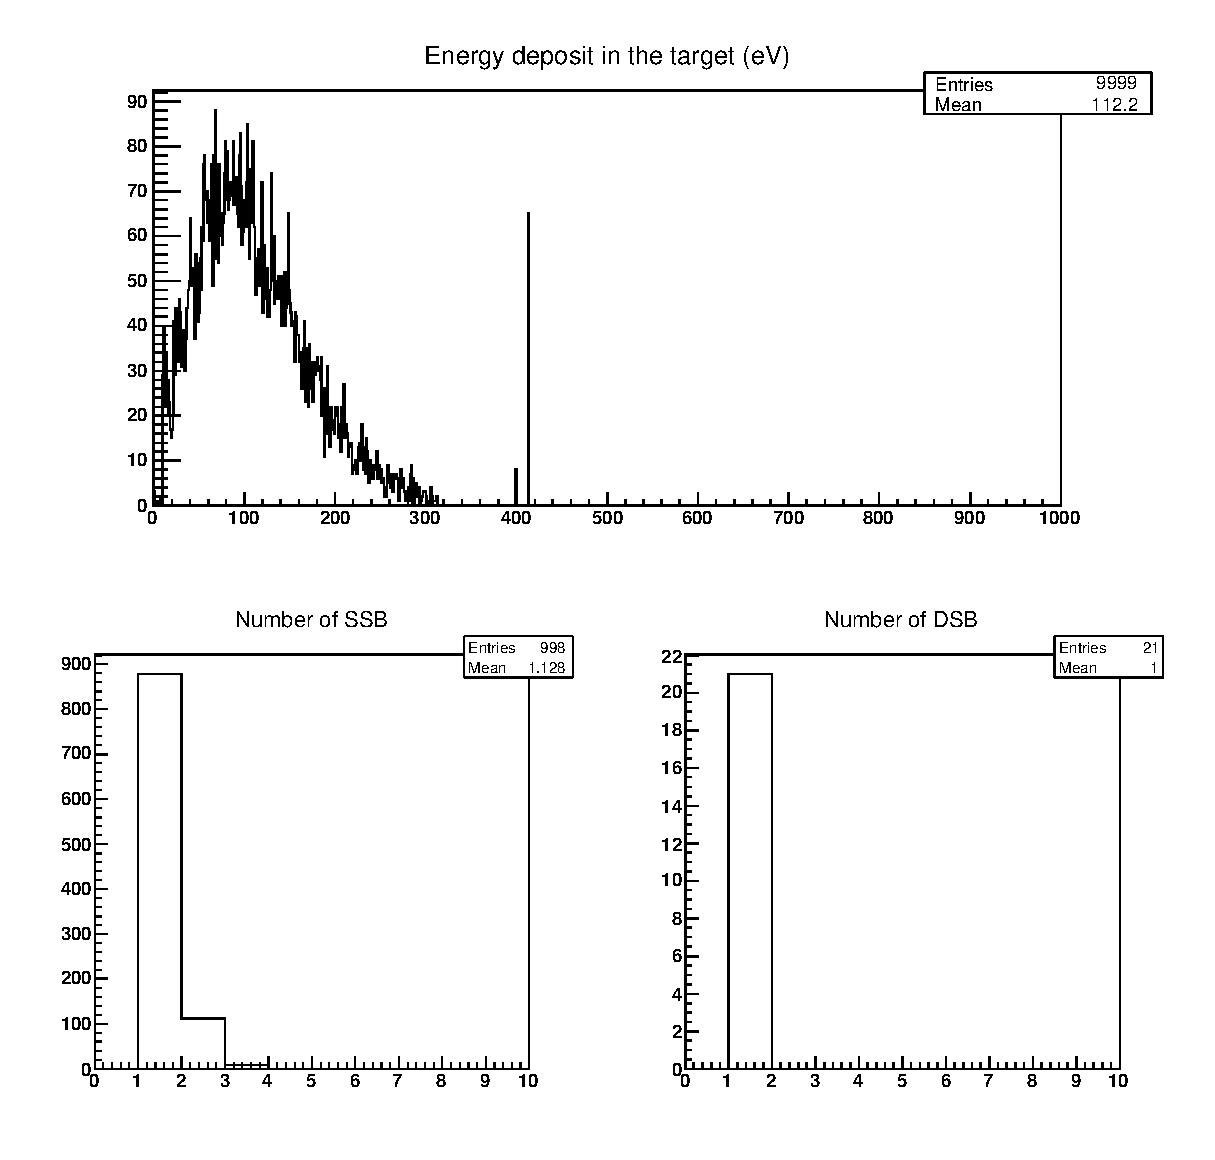
\includegraphics[width=.78\linewidth]{./Figures/proton400eV.eps}
%  \caption{400 eV}
%  \label{fig:sub2}
%\end{subfigure}
%\begin{subfigure}{.5\textwidth}
%  \centering
%  \includegraphics[width=.78\linewidth]{./Figures/proton600eV.eps}
%  \caption{600 eV}
%  \label{fig:sub3}
%\end{subfigure}%
%\begin{subfigure}{.5\textwidth}
%  \centering
%  \includegraphics[width=.78\linewidth]{./Figures/proton800eV.eps}
%  \caption{800 eV}
%  \label{fig:sub4}
%\end{subfigure}
%\begin{subfigure}{.5\textwidth}
%  \centering
%  \includegraphics[width=.78\linewidth]{./Figures/proton1kev.eps}
%  \caption{1 keV}
%  \label{fig:sub5}
%\end{subfigure}%
%\begin{subfigure}{.5\textwidth}
%  \centering
%  \includegraphics[width=.78\linewidth]{./Figures/proton200kev.eps%}
%  \caption{200 keV}
%  \label{fig:sub6}
%\end{subfigure}
%\begin{subfigure}{.5\textwidth}
%  \centering
%  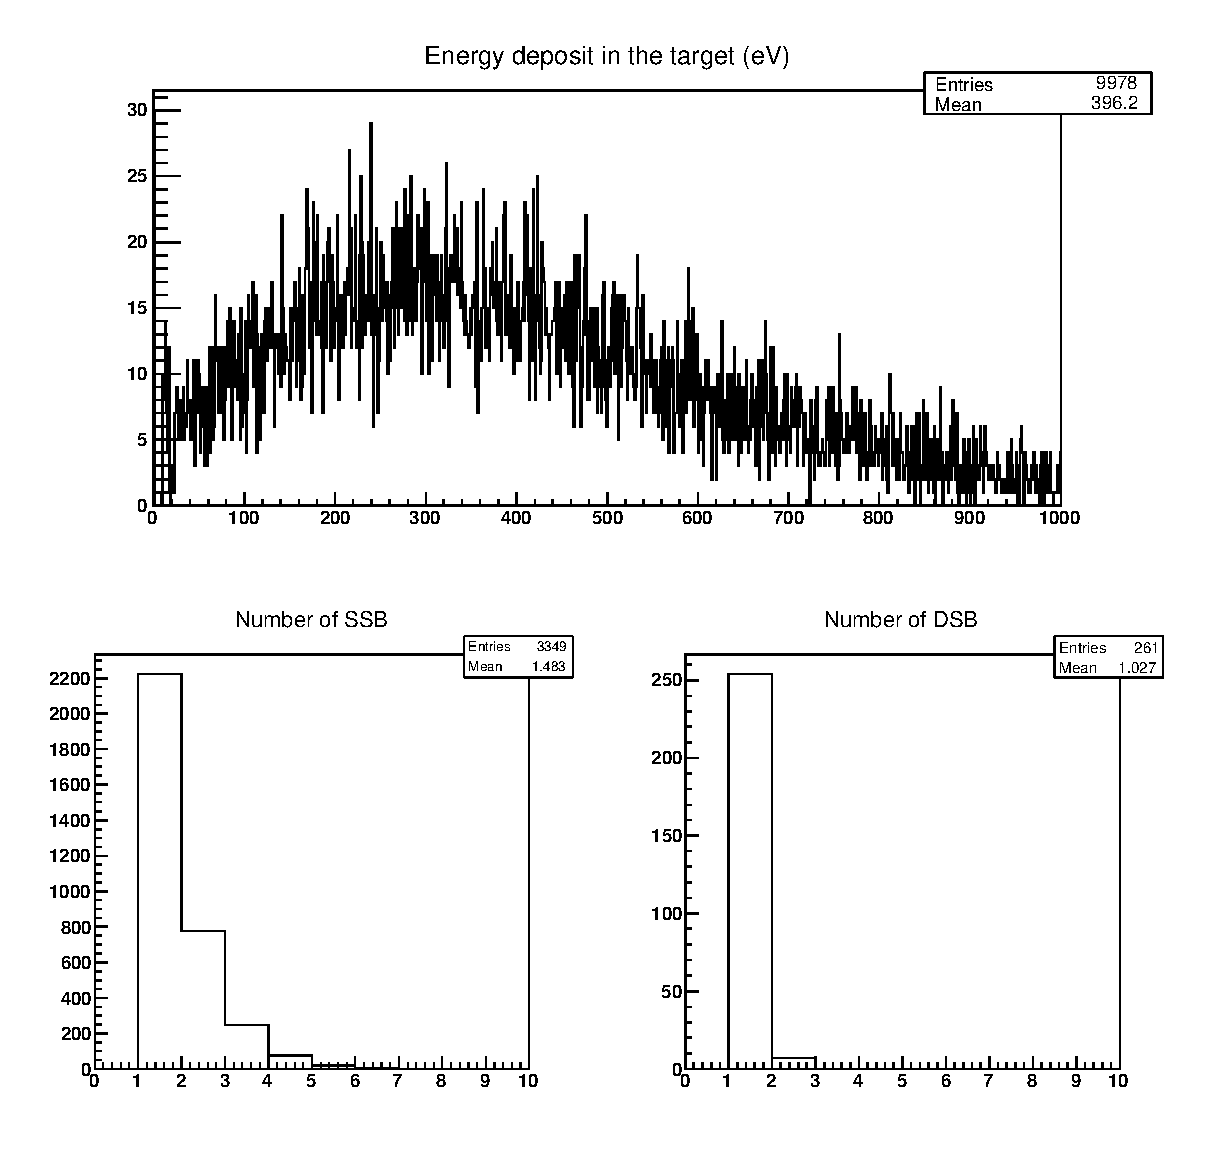
\includegraphics[width=.78\linewidth]{./Figures/proton400kev.eps%}
%  \caption{400 keV}
%  \label{fig:sub7}
%\end{subfigure}%
%\begin{subfigure}{.5\textwidth}
%  \centering
%  \includegraphics[width=.78\linewidth]{./Figures/proton600kev.eps%}
%  \caption{600 keV}
%  \label{fig:sub8}
%\end{subfigure}
%\caption{Rompimientos simples y dobles para 1ZBB ($proton$)}
%\label{fig:p}
%\end{figure}
%
%\clearpage
%\section{Anexo}
%\label{ede3}
%
%
%
%\begin{figure}
%\centering
%\begin{subfigure}{.5\textwidth}
%  \centering
%  \includegraphics[width=.78\linewidth]{./Figures/040.eps}
%  \caption{40 eV}
%  \label{fig:sube1}
%\end{subfigure}%
%\begin{subfigure}{.5\textwidth}
%  \centering
%  \includegraphics[width=.78\linewidth]{./Figures/1.eps}
%  \caption{100 eV}
%  \label{fig:sube2}
%\end{subfigure}
%\begin{subfigure}{.5\textwidth}
%  \centering
%  \includegraphics[width=.78\linewidth]{./Figures/2.eps}
%  \caption{200 eV}
%  \label{fig:sube3}
%\end{subfigure}%
%\begin{subfigure}{.5\textwidth}
%  \centering
%  \includegraphics[width=.78\linewidth]{./Figures/3.eps}
%  \caption{400 eV}
%  \label{fig:sube4}
%\end{subfigure}
%\begin{subfigure}{.5\textwidth}
%  \centering
%  \includegraphics[width=.78\linewidth]{./Figures/4.eps}
%  \caption{600 eV}
%  \label{fig:sube5}
%\end{subfigure}%
%\begin{subfigure}{.5\textwidth}
%  \centering
%  \includegraphics[width=.78\linewidth]{./Figures/5.eps}
%  \caption{800 eV}
%  \label{fig:sube6}
%\end{subfigure}
%\begin{subfigure}{.5\textwidth}
%  \centering
%  \includegraphics[width=.78\linewidth]{./Figures/6.eps}
%  \caption{1 keV}
%  \label{fig:sube7}
%\end{subfigure}%
%\begin{subfigure}{.5\textwidth}
%  \centering
%  \includegraphics[width=.78\linewidth]{./Figures/7.eps}
%  \caption{20 keV}
%  \label{fig:sube8}
%\end{subfigure}
%\caption{Rompimientos simples y dobles para 1FZX ($e-$)}
%\label{fig:e2}
%\end{figure}
%
%
%\clearpage
%\section{Anexo}
%\label{ede4}
%
%
%\begin{figure}
%\centering
%\begin{subfigure}{.5\textwidth}
%  \centering
%  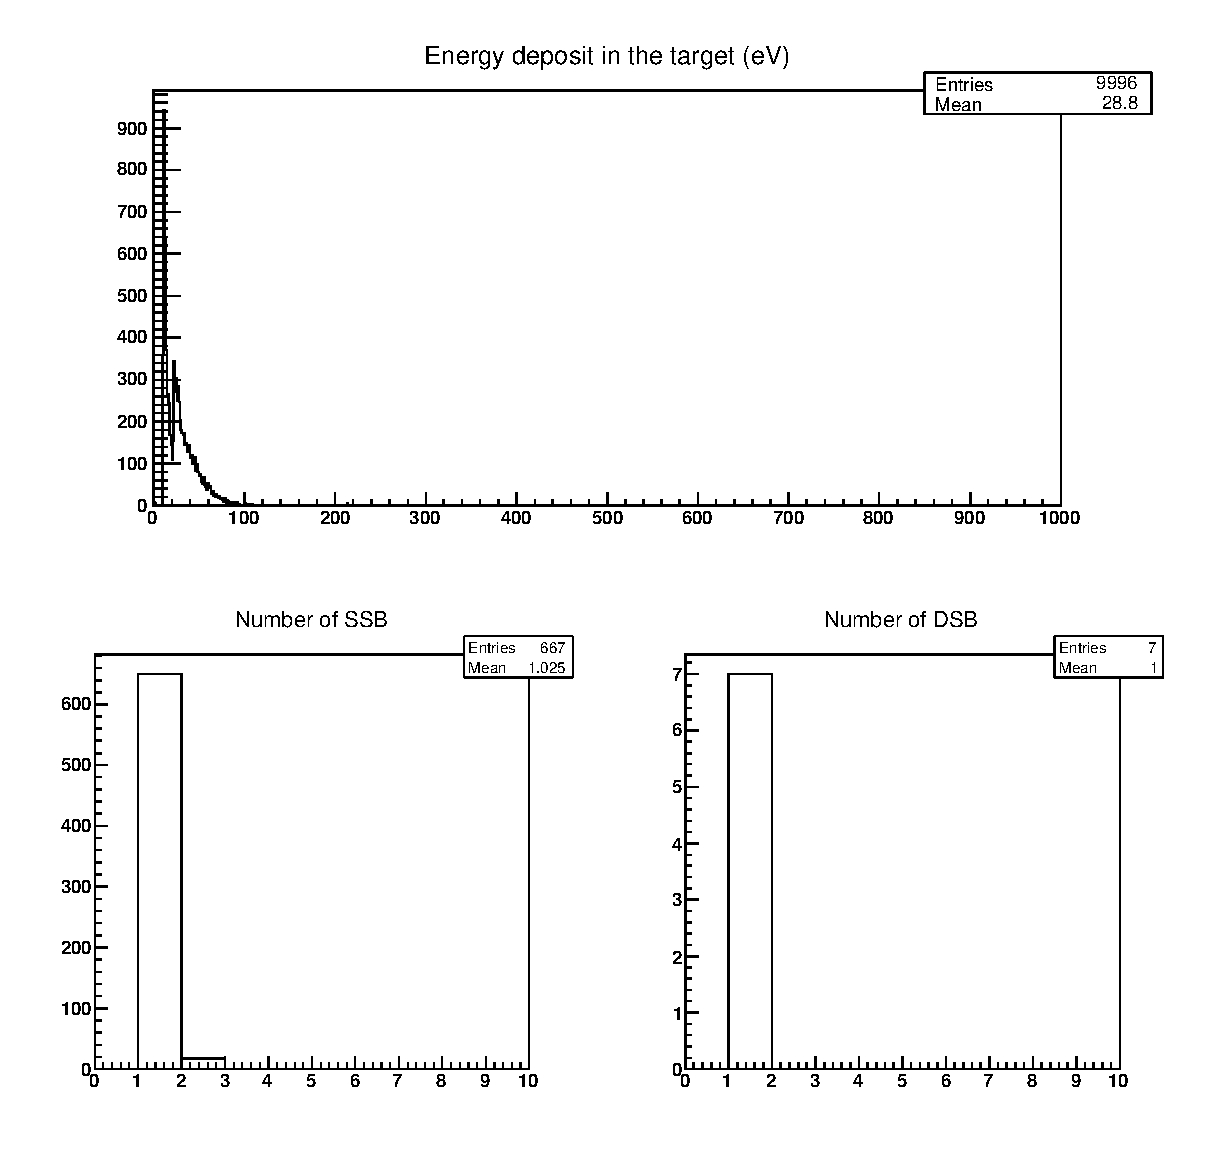
\includegraphics[width=.78\linewidth]{./Figures/11.eps}
%  \caption{200 eV}
%  \label{fig:subi1}
%\end{subfigure}%
%\begin{subfigure}{.5\textwidth}
%  \centering
%  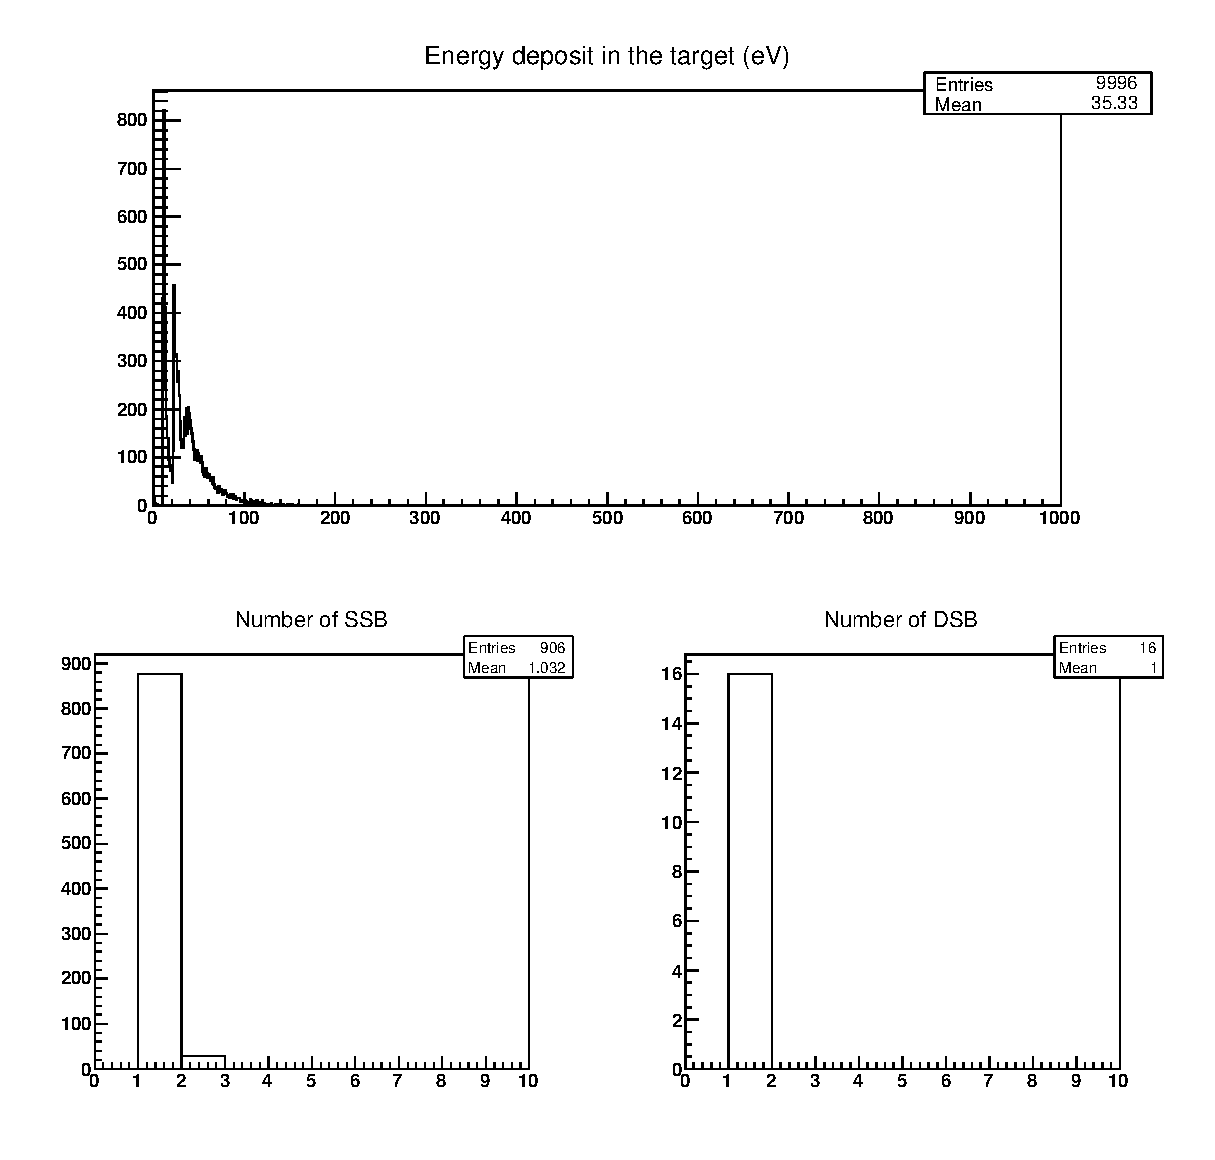
\includegraphics[width=.78\linewidth]{./Figures/22.eps}
%  \caption{400 eV}
%  \label{fig:subi2}
%\end{subfigure}
%\begin{subfigure}{.5\textwidth}
%  \centering
%  \includegraphics[width=.78\linewidth]{./Figures/33.eps}
%  \caption{600 eV}
%  \label{fig:subi3}
%\end{subfigure}%
%\begin{subfigure}{.5\textwidth}
%  \centering
%  \includegraphics[width=.78\linewidth]{./Figures/44.eps}
%  \caption{800 eV}
%  \label{fig:subi4}
%\end{subfigure}
%\begin{subfigure}{.5\textwidth}
%  \centering
%  \includegraphics[width=.78\linewidth]{./Figures/55.eps}
%  \caption{1 keV}
%  \label{fig:subi5}
%\end{subfigure}%
%\begin{subfigure}{.5\textwidth}
%  \centering
%  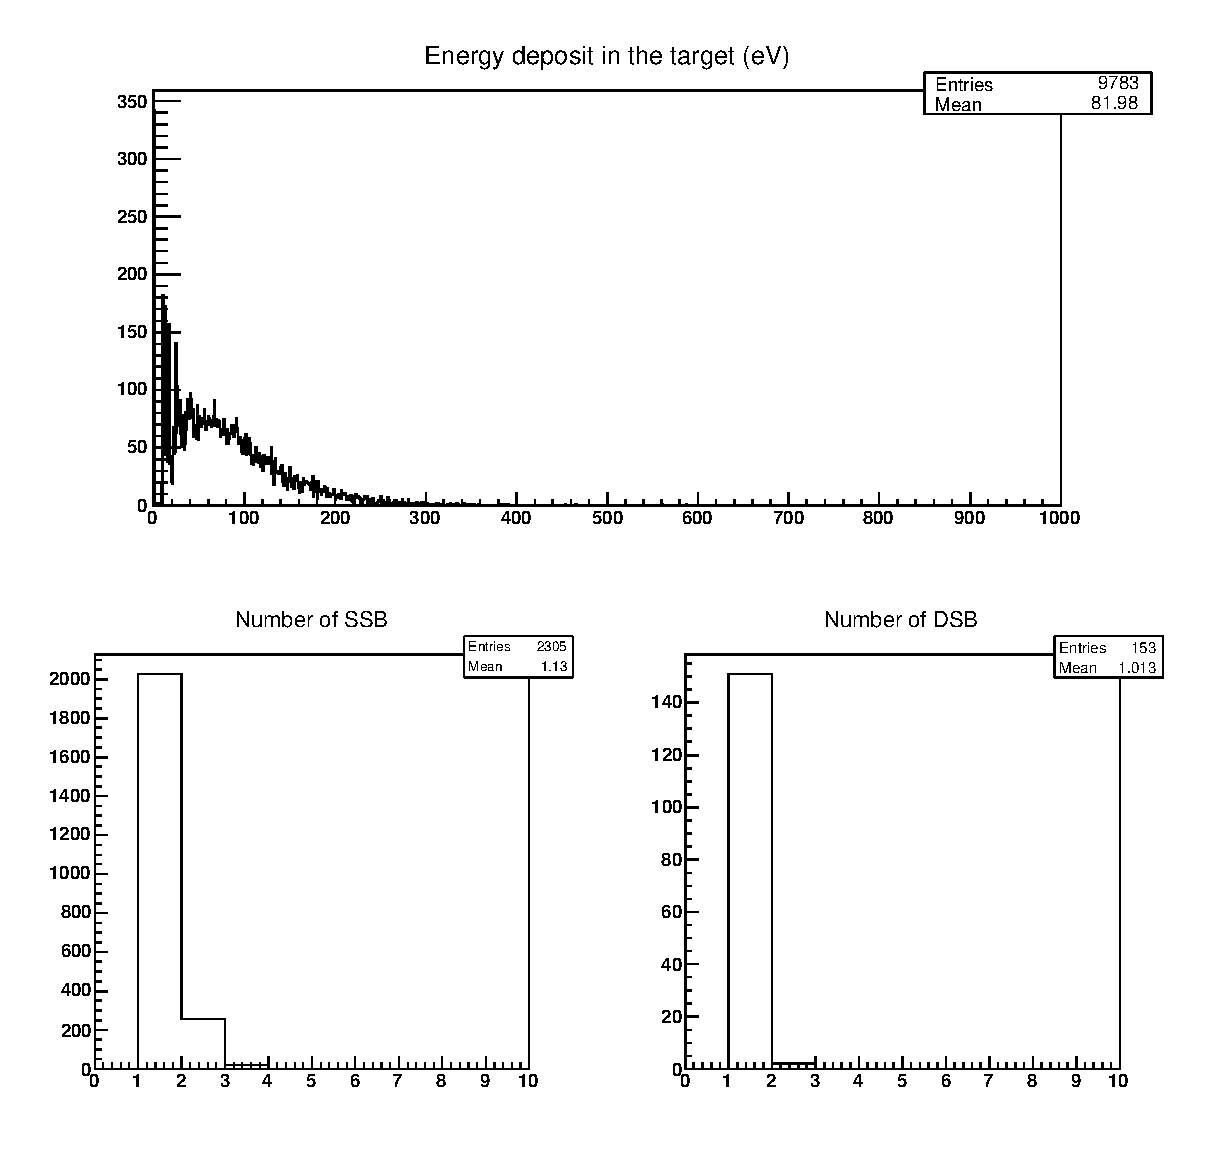
\includegraphics[width=.78\linewidth]{./Figures/66.eps}
%  \caption{200 keV}
%  \label{fig:subi6}
%\end{subfigure}
%\begin{subfigure}{.5\textwidth}
%  \centering
%  \includegraphics[width=.78\linewidth]{./Figures/77.eps}
%  \caption{400 keV}
%  \label{fig:subi7}
%\end{subfigure}%
%\begin{subfigure}{.5\textwidth}
%  \centering
%  \includegraphics[width=.78\linewidth]{./Figures/88.eps}
%  \caption{600 keV}
%  \label{fig:subi8}
%\end{subfigure}
%\caption{Rompimientos simples y dobles para 1FZX ($proton$)}
%\label{fig:p2}
%\end{figure}
%
%
\clearpage
\section{Anexo}
\label{app:M}
\lstset {language=C++}
\begin{lstlisting}
      double TotalMass = 0.0;
      double TotalMassPhosResSeq1 = 0.0;
      double TotalMassSugResSeq1 = 0.0;
      double TotalMassBaseResSeq1 = 0.0;
      double TotalMassPhosResSeq2 = 0.0;
      double TotalMassSugResSeq2 = 0.0;
      double TotalMassBaseResSeq2 = 0.0;


      for(int i = 0; i < residueListTemp->fNbAtom; i++)
      {
	//EM
      	//////////////////////////////////////
	// Set Mass expressed in u
        double ElementMass = 0.0;
        if(AtomTemp->fElement == "H") ElementMass = 1.00784;
	else if(AtomTemp->fElement == "C") ElementMass = 12.0107;
        else if(AtomTemp->fElement == "N") ElementMass = 14.0067;
        else if(AtomTemp->fElement == "O") ElementMass = 15.999;
        else if(AtomTemp->fElement == "P") ElementMass = 30.973762;
        else if(AtomTemp->fElement == "S") ElementMass = 32.065;
        else
	  {
          G4cerr << "Element not recognized : " << AtomTemp->fElement << G4endl;
          G4cerr << "Stop now" << G4endl;
          exit(1);
        }
\end{lstlisting}

\clearpage
\section{Anexo}
\label{app:CM}
\lstset {language=C++}
\begin{lstlisting}
//Center of mass calculation
else if( OptCalc == 2 )
  {
    baryX += ElementMass * (AtomTemp->fX);
    baryY += ElementMass * (AtomTemp->fY);
    baryZ += ElementMass * (AtomTemp->fZ);
    TotalMass += ElementMass;

    if(residueListTemp->fResSeq == 1)
      {
  if(i == 0)
    {
      baryPhosX += ElementMass * (AtomTemp->fX);
      baryPhosY += ElementMass * (AtomTemp->fY);
      baryPhosZ += ElementMass * (AtomTemp->fZ);
      TotalMassPhosResSeq1 += ElementMass;
    }
  else if(i < 8)
    {
      barySugX += ElementMass * (AtomTemp->fX);
      barySugY += ElementMass * (AtomTemp->fY);
      barySugZ += ElementMass * (AtomTemp->fZ);
      TotalMassSugResSeq1 += ElementMass;
    }
  else
    {
      //hydrogen are placed at the end of the residue in a PDB file
      //We don't want them for this calculation
      if(AtomTemp->fElement != "H")
        {
    baryBaseX += ElementMass * (AtomTemp->fX);
    baryBaseY += ElementMass * (AtomTemp->fY);
    baryBaseZ += ElementMass * (AtomTemp->fZ);
    TotalMassBaseResSeq1 += ElementMass;
        }
    }
      } //// if(residueListTemp->fResSeq == 1)........
    else  //if(residueListTemp->fResSeq != 1)
      {
  if(i < 4)
    {
      baryPhosX += ElementMass * (AtomTemp->fX);
      baryPhosY += ElementMass * (AtomTemp->fY);
      baryPhosZ += ElementMass * (AtomTemp->fZ);
      TotalMassPhosResSeq2 += ElementMass;
    }
  else if(i < 11)
    {
      barySugX += ElementMass * (AtomTemp->fX);
      barySugY += ElementMass * (AtomTemp->fY);
      barySugZ += ElementMass * (AtomTemp->fZ);
      TotalMassSugResSeq2 += ElementMass;
    }
  else
    {
      //hydrogen are placed at the end of the residue in a PDB file
      //We don't want them for this calculation
      if(AtomTemp->fElement != "H")
        { // break;
    baryBaseX += ElementMass * (AtomTemp->fX);
    baryBaseY += ElementMass * (AtomTemp->fY);
    baryBaseZ += ElementMass * (AtomTemp->fZ);
    TotalMassBaseResSeq2 += ElementMass;
        }
    }
      } // //if(residueListTemp->fResSeq != 1).......
  } //else if( OptCalc == 2 ).....
//Neither OpcCalc=1 nor OptCalc=2
else
  G4cerr << "Something is fishy!! : "  << G4endl;
AtomTemp = AtomTemp->GetNext();
    } //end of for (  i=0 ; i < residueListTemp->nbAtom ; i++)
\end{lstlisting}
